\documentclass[unicode,a4paper,11pt]{ltjsarticle}

\usepackage{luatexja-fontspec}
\setmainfont{TeX Gyre Termes}
% \setmainjfont[BoldFont = IPAGothic]{IPAMincho}
\setmathrm{Latin Modern Roman}
\setmainjfont{Noto Sans JP}

% ---Display \subsubsection at the Index
% \setcounter{tocdepth}{3}

% ---Setting about the geometry of the document----
% \usepackage{a4wide}
% \pagestyle{empty}

% ---Physics and Math Packages---
\usepackage{amssymb,amsfonts,amsthm,mathtools}
\usepackage{physics,braket,bm}

% ---underline---
\usepackage[normalem]{ulem}

% ---cancel---
\usepackage{cancel}

% --- surround the texts or equations
% \usepackage{fancybox,ascmac}

% ---settings of theorem environment---
% \usepackage{amsthm}
% \theoremstyle{definition}

% ---settings of proof environment---
% \renewcommand{\proofname}{\textbf{証明}}
% \renewcommand{\qedsymbol}{$\blacksquare$}

% ---Ignore the Warnings---
\usepackage{silence}
\WarningFilter{latexfont}{Some font shapes}
\WarningFilter{latexfont}{Font shape}
\WarningFilter{latexfont}{Size substitutions}
\ExplSyntaxOn
\msg_redirect_name:nnn{hooks}{generic-deprecated}{none}
\ExplSyntaxOff

% ---Insert the figure (If insert the `draft' at the option, the process becomes faster.)---
\usepackage{graphicx}
% \usepackage{subcaption}

% ----Add a link to a text---
\usepackage{url,hyperref}
\usepackage[dvipsnames,svgnames]{xcolor}
\hypersetup{colorlinks=true,citecolor=FireBrick,linkcolor=Navy,urlcolor=purple}
% ---refer `texdoc xcolor' at the command line---

% ---Tikz---
% \usepackage{tikz,pgf,pgfplots,circuitikz}
% \pgfplotsset{compat=1.15}
% \usetikzlibrary{intersections,arrows.meta,angles,calc,3d,decorations.pathmorphing}

% ---Add the section number to the equation, figure, and table number---
\makeatletter
   \renewcommand{\theequation}{\thesection.\arabic{equation}}
   \@addtoreset{equation}{section}
   
   \renewcommand{\thefigure}{\thesection.\arabic{figure}}
   \@addtoreset{figure}{section}
   
   \renewcommand{\thetable}{\thesection.\arabic{table}}
   \@addtoreset{table}{section}
\makeatother

% ---enumerate---
% \renewcommand{\labelenumi}{$\arabic{enumi}.$}
% \renewcommand{\labelenumii}{$(\arabic{enumii})$}

% ---Index---
% \usepackage{makeidx}
% \makeindex 

% ---Fonts---
% \renewcommand{\familydefault}{\sfdefault}

% ---Title---
\title{
    2024年度\ 春の学校\ しおり\ v1
}
\author{
  校長:宮根
}
\date{最終更新:\today}

\begin{document}

\maketitle

* This document is the handbook about the spring seminar. The English version begins from page \pageref{eng_page}.

\tableofcontents



\clearpage

\section{スケジュール}

\begin{center}
  \begin{tabular}{cll}\hline
    日        & 時間                 & 予定                                      \\ \hline
    4/6\ (土) & 13:00                & セミナーハウス到着                        \\
              &                      & 荷物を部屋において、ゼミ室へ。            \\
              & 13:20                & 発表開始                                  \\
              & 16:30                & 発表終了                                  \\
              &                      & 入浴など。                                \\
              & 18:00\ $\sim$\ 19:00 & 夕食                                      \\
              & 19:00\ $\sim$\ 22:00 & 宴会                                      \\
              &                      & (片づけを含めた時間)                      \\
              & 23:00                & 就寝                                      \\ \hline
    4/7\ (日) & 7:00                 & 起床                                      \\
              & 7:30\ $\sim$\  8:30  & 朝食                                      \\
              & 9:00                 & チェックアウト\ \&\ 発表開始              \\
              & 11:40                & 発表終了                                  \\
              &                      & お茶会・写真撮影など\ $\rightarrow$\ 解散 \\ \hline
  \end{tabular}
\end{center}

\begin{itemize}
  \item
        入浴ができるのは16:00\ $\sim$\ 22:00です。
  \item
        食事は上記の時間内に済ませてください。
  \item
        一応、チェックアウトは10:00までです。
  \item
        去年は(買い出し班が)少し早めに到着したら怒られました。
\end{itemize}

\section{発表タイムテーブル}

\begin{center}
  \begin{tabular}{clcl}\hline
    日        & 時間                 & 発表時間\ (分) & 発表者            \\ \hline
    4/6\ (土) & 13:20\ $\sim$\ 13:45 & 25             & 安倍 博之\ (教授) \\
              & 13:50\ $\sim$\ 14:30 & 40             & 小市 明勢\ (M)    \\
              & 14:35\ $\sim$\ 15:15 & 40             & 永井 駿平\ (M)    \\
              & 15:15\ $\sim$\ 15:30 &                & (15分\ 休憩)      \\
              & 15:30\ $\sim$\ 15:40 & 10             & 嶋田 直希\ (M)    \\
              & 15:45\ $\sim$\ 15:55 & 10             & 宮根 一樹\ (M)    \\
              & 16:00\ $\sim$\ 16:30 & 30             & Raiyan Haque\ (B) \\ \hline
    4/7\ (日) & 9:00\ $\sim$\ 9:25   & 25             & 中里 弘道\ (教授) \\
              & 9:30\ $\sim$\ 9:40   & 10             & 落合 誠\ (助教)   \\
              & 9:45\ $\sim$\ 9:55   & 10             & 渡辺 あかね\ (D)  \\
              & 10:00\ $\sim$\ 10:10 & 10             & 徳永 尚文\ (D)    \\
              & 10:10\ $\sim$\ 10:30 &                & (20分\ 休憩)      \\
              & 10:30\ $\sim$\ 10:40 & 10             & 岩村 海飛\ (D)    \\
              & 10:45\ $\sim$\ 11:25 & 40             & 谷口 永希\ (M)    \\
              & 11:30\ $\sim$\ 11:40 & 10             & 芝山 駿介\ (M)    \\ \hline
  \end{tabular}
\end{center}

\begin{itemize}
  \item
        発表時間は\textbf{質疑応答込み}の時間です。タイムキーピングをお願いします。
\end{itemize}

\section{部屋割り}

\begin{center}
  \begin{tabular}{cl}\hline
    部屋番号 & メンバー                                      \\ \hline
    301      & 中里 弘道                                     \\
    302      & 安倍 博之                                     \\
    303      & 渡辺 あかね                                   \\
    202      & 岩村 海飛、 徳永 尚文、落合 誠、永井 駿平     \\
    203      & 小市 明勢、 谷口 永希、宮根 一樹、嶋田 直希   \\
    204      & 芝山 駿介、 佐久間 紀丞、下田 幹人、堀内 嵩真 \\
    205      & 花村 晃、吉田 聡一郎、Raiyan Haque            \\ \hline
  \end{tabular}
\end{center}

\begin{itemize}
  \item
        従わなくて結構です。
  \item
        宿泊部屋での飲酒は禁止だそうです。
\end{itemize}


\section{電車利用の際の参考経路}

\vspace*{5pt}

\begin{center}
  \begin{minipage}[ht]{0.48\columnwidth}
    \textbf{通常班}

    \vspace*{5pt}

    \begin{tabular}{cl}\hline
      時間     &                                 \\ \hline
      9:55 発  & 高田馬場                        \\
               & $\downarrow$\ JR\ 山手線        \\
      10:20 着 & 品川                            \\
      10:34 発 &                                 \\
               & $\downarrow$\ JR\ こだま\ 717号 \\
      11:12 着 & 熱海                            \\
      11:32 発 &                                 \\
               & $\downarrow$\ JR\ 伊東線        \\
      12:05 着 & 川奈                            \\ \hline
    \end{tabular}
  \end{minipage}
  \begin{minipage}[ht]{0.48\columnwidth}
    \textbf{買い出し班}

    \vspace*{5pt}

    \begin{tabular}{cl}\hline
      時間     &                                 \\ \hline
      8:54 発  & 高田馬場                        \\
               & $\downarrow$\ JR\ 山手線        \\
      9:18 着  & 品川                            \\
      9:34 発  &                                 \\
               & $\downarrow$\ JR\ こだま\ 717号 \\
      10:10 着 & 熱海                            \\
      10:45 発 &                                 \\
               & $\downarrow$\ JR\ 伊東線        \\
      11:16 着 & 川奈                            \\ \hline
    \end{tabular}
  \end{minipage}
\end{center}

\begin{itemize}
  \item
        料金はいずれも4,410円です。
  \item
        (特急を除けば、)買い出し班と通常班の間には電車がありません。
  \item
        通常班も熱海11:32発の電車を逃したら、次は12:24発になります。
\end{itemize}

\section{その他・注意事項}





\clearpage

\setcounter{section}{0}

Here is the English version. Since I spent a lot of time making this version, I hope some English students to read this eagerly.

\label{eng_page}

\section{Schedule}

\begin{center}
  \begin{tabular}{cll}\hline
    Date          & Time               & Schedule                                           \\ \hline
    Sat. Apr. 6th & 1:00 p.m.          & Arrive at seminar house                            \\
                  &                    & Put loads in the room and move to the seminar room \\
                  & 1:20               & Start presentation                                 \\
                  & 4:30               & End                                                \\
                  &                    & bathe, etc.                                        \\
                  & 6:00  $\sim$ 7:00  & Dinner                                             \\
                  & 7:00  $\sim$ 10:00 & Party                                              \\
                  &                    & (Clean up by 10:00 p.m.)                           \\
                  & 11:00 p.m.         & Go to bed                                          \\ \hline
    Sun. Apr. 7th & 7:00 a.m.          & Get up                                             \\
                  & 7:30 $\sim$  8:30  & Breakfast                                          \\
                  & 9:00               & Complete check out\ \&\ Start presentation         \\
                  & 11:40 a.m.         & End                                                \\
                  &                    & Tea time, Photo, etc.\ $\rightarrow$\ Breakup!     \\ \hline
  \end{tabular}
\end{center}

\begin{itemize}
  \item
        Bathing is from  4:00 p.m. to 10:00 p.m.
  \item
        Meals should be finished by the time mentioned above.
  \item
        Checkout is by 10:00 a.m.
  \item
        In the last year, we made the director of the seminar house angry since some students arrived earlier.
\end{itemize}


\section{Timetable}

\begin{center}
  \begin{tabular}{clcl}\hline
    Date          & Time                      & Presentation time\ (min) & Presenter                        \\ \hline
    Sat. Apr. 6th & 1:20 p.m.\ $\sim$\ 1:45   & 25                       & Hiroyuki Abe\ (Professor)        \\
                  & 1:50\ $\sim$\ 2:30        & 40                       & Akinari Koichi\ (M)              \\
                  & 2:35\ $\sim$\ 3:15        & 40                       & Shunpei Nagai\ (M)               \\
                  & 3:15\ $\sim$\ 3:30        &                          & (15 min break)                   \\
                  & 3:30\ $\sim$\ 3:40        & 10                       & Naoki Shimada\ (M)               \\
                  & 3:45\ $\sim$\ 3:55        & 10                       & Itsuki Miyane\ (M)               \\
                  & 4:00\ $\sim$\ 4:30 p.m.   & 30                       & Raiyan Haque\ (B)                \\ \hline
    Sun. Apr. 7th & 9:00 a.m \ $\sim$\ 9:25   & 25                       & Hiromichi Nakazato\ (Professor)  \\
                  & 9:30\ $\sim$\ 9:40        & 10                       & Makoto Ochiai\ (Assistant Prof.) \\
                  & 9:45\ $\sim$\ 9:55        & 10                       & Akane Watanabe\ (D)              \\
                  & 10:00\ $\sim$\ 10:10      & 10                       & Takafumi Tokunaga\ (D)           \\
                  & 10:10\ $\sim$\ 10:30      &                          & (20 min break)                   \\
                  & 10:30\ $\sim$\ 10:40      & 10                       & Kaito Iwamura\ (D)               \\
                  & 10:45\ $\sim$\ 11:25      & 40                       & Eiki Taniguchi\ (M)              \\
                  & 11:30\ $\sim$\ 11:40 a.m. & 10                       & Shunsuke Shibayama\ (M)          \\ \hline
  \end{tabular}
\end{center}

\begin{itemize}
  \item
        Presentation time includes Q\&A sessions. Please be careful not to extend.
\end{itemize}

\section{Room Allocation}

\begin{center}
  \begin{tabular}{cl}\hline
    Room Number & Member                                                            \\ \hline
    301         & Hiromichi Nakazato                                                \\
    302         & Hiroyuki Abe                                                      \\
    303         & Akane Watanabe                                                    \\
    202         & Kaito Iwamura, Takafumi Tokunaga, Makoto Ochiai, Shunpei Nagai    \\
    203         & Akinari Koichi, Eiki Taniguchi, Itsuki Miyane, Naoki Shimada      \\
    204         & Shunsuke Shibayama, Kisuke Sakuma, Mikito Shimoda, Shuma Horiuchi \\
    205         & Akira Hanamura, Soichiro Yoshida, Raiyan Haque                    \\ \hline
  \end{tabular}
\end{center}

\begin{itemize}
  \item
        You shouldn't follow the table above.
  \item
        It is \textit{not} permitted to drink alcohol in the room.
\end{itemize}


\section{Example of Transfers}

\vspace*{5pt}

\begin{center}
  \begin{minipage}[ht]{0.48\columnwidth}
    \textbf{Normal Team}

    \vspace*{5pt}

    \begin{tabular}{cl}\hline
      Time           &                                 \\ \hline
      From 9:55 a.m. & Takadanobaba                    \\
                     & $\downarrow$\ JR\ Yamanote line \\
      To 10:20       & Shinagawa                       \\
      From 10:34     &                                 \\
                     & $\downarrow$\ JR\ Kodama\ 717   \\
      To 11:12       & Atami                           \\
      From 11:32     &                                 \\
                     & $\downarrow$\ JR\ Ito line      \\
      To 12:05       & Kawana                          \\ \hline
    \end{tabular}
  \end{minipage}
  \begin{minipage}[ht]{0.48\columnwidth}
    \textbf{Grocery Shopping Team}

    \vspace*{5pt}

    \begin{tabular}{cl}\hline
      Time           &                                 \\ \hline
      From 8:54 a.m. & Takadanobaba                    \\
                     & $\downarrow$\ JR\ Yamanote line \\
      To 9:18        & Shinagawa                       \\
      From 9:34      &                                 \\
                     & $\downarrow$\ JR\ Kodama\ 717   \\
      To 10:10       & Atami                           \\
      From 10:45     &                                 \\
                     & $\downarrow$\ JR\ Ito line      \\
      To 11:16       & Kawana                          \\ \hline
    \end{tabular}
  \end{minipage}
\end{center}

\begin{itemize}
  \item
        It costs 4,410 Yen for both courses.
  \item
        There is no train between the normal team and the shopping team from Atami station. So we can't be late. I will try my best.
  \item
        By the way, if the normal team member misses the train from 11:32 a.m., he or she has to take the train from 12:24 p.m. There are fewer trains in Shizuoka than in Tokyo.
\end{itemize}


\section{Notes}






\clearpage

\section{リンク集 / Links}

\begin{itemize}
  \item
        \href{https://www.waseda.jp/inst/student/facility/seminar/facility/izukawana}{ホームページ / Webpage}
  \item
        \href{https://www.waseda.jp/inst/student/facility/seminar/flow/tips}{利用上の心得 / Usage tips}
\end{itemize}

\section{懇親会 / Konshinkai}

こんなのが引継ぎのフォルダにありました。

I found the following in the shared folder.

\begin{center}
  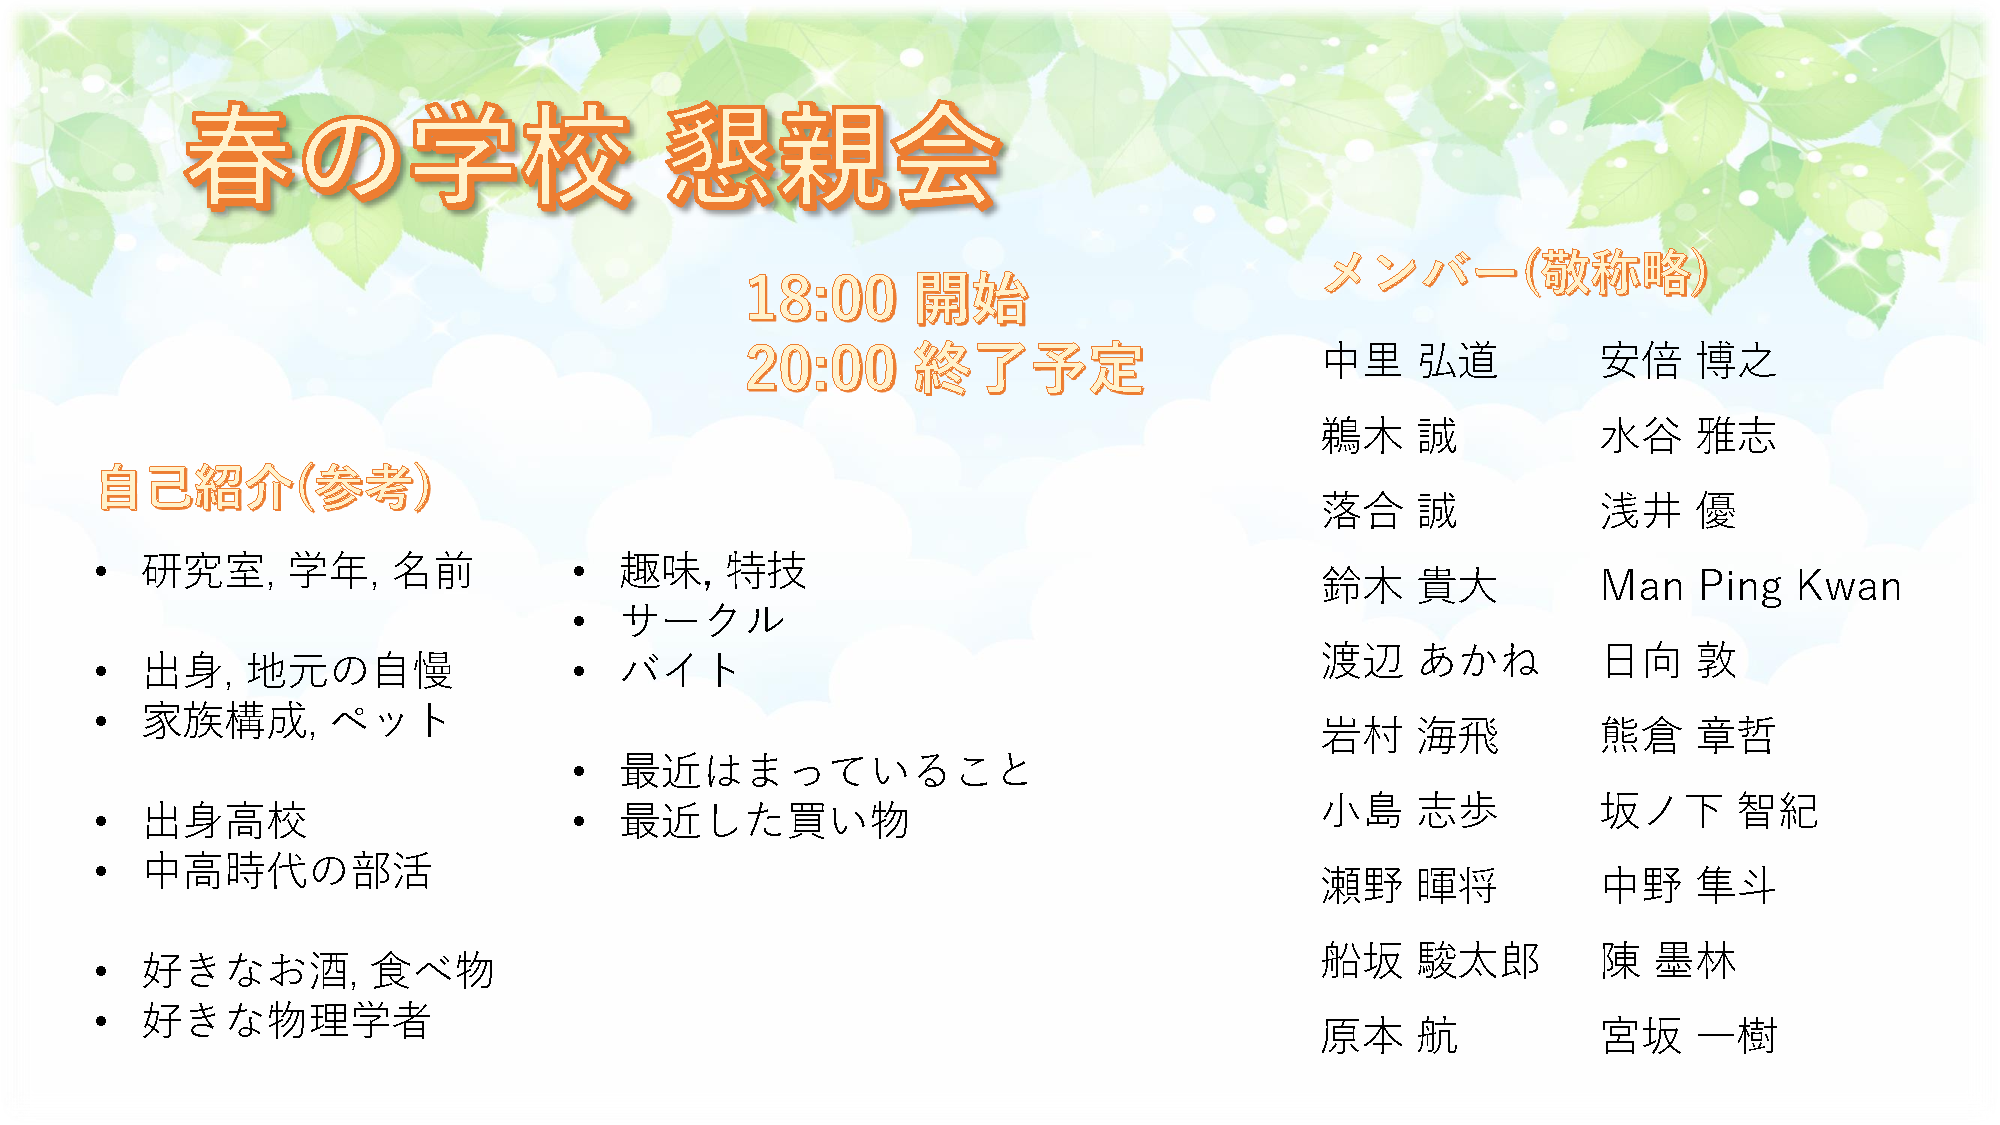
\includegraphics[width=1.0\linewidth]{konshinkai.pdf}
\end{center}



\end{document}
